%!TEX root = ../crimson_throne_book_main.tex
% 2016-02-27
To a man dressed in shiny armor rust monsters inspire a fair amount of fear, more so than a mantidrake or three terror birds, who are in fact fiercer opponents. Quint {\itshape hastes} his friends and makes for the stairs at the end of the room, drawing away the  {\itshape invisibility} from anyone but himself. Waiting at the top of the wooden steps is another nasty surprise: orcs! Meanwhile Sjo, Puk and Spyder take care of the rust eating beasts with ease, while Balian tanks the terror birds. Uri, the little orc guide, hides under the table and just watches what happens. Quint presses up against the wall as the orcs from above charge down. Still, one of them, who looks the smartest and probably has the keenest senses, spots the invisible bard on the stairs and stabs him with his dagger. {\itshape``You see,}'' he screams, {\itshape``the purple worm was right, he wasn't alone!}'' Sjo rushes past the mantidrake to give Puk flanking, allowing the halfling to cut down the creature in a matter of seconds. By now two orcs have joined the fight on the ground floor, one is engaging Quint on the stairs, while two more archers appear and fire upon Sjo. Their arrows fail to pierce his armor.\hyperref[fig:Orc-ambush-in-Urgir-593345070]{ Despite the number of opponents, the fight turns out to be easy. } The enemy has a hard time wounding the party and one by one the birds and orcs go down. The dagger-wielding leader of the orcs tries to make a run for it, but is literally held  in place by Sjo's magic. The heroes disarm him and lock him up in a small cage. \\

\begin{figure}[h]
	\centering
	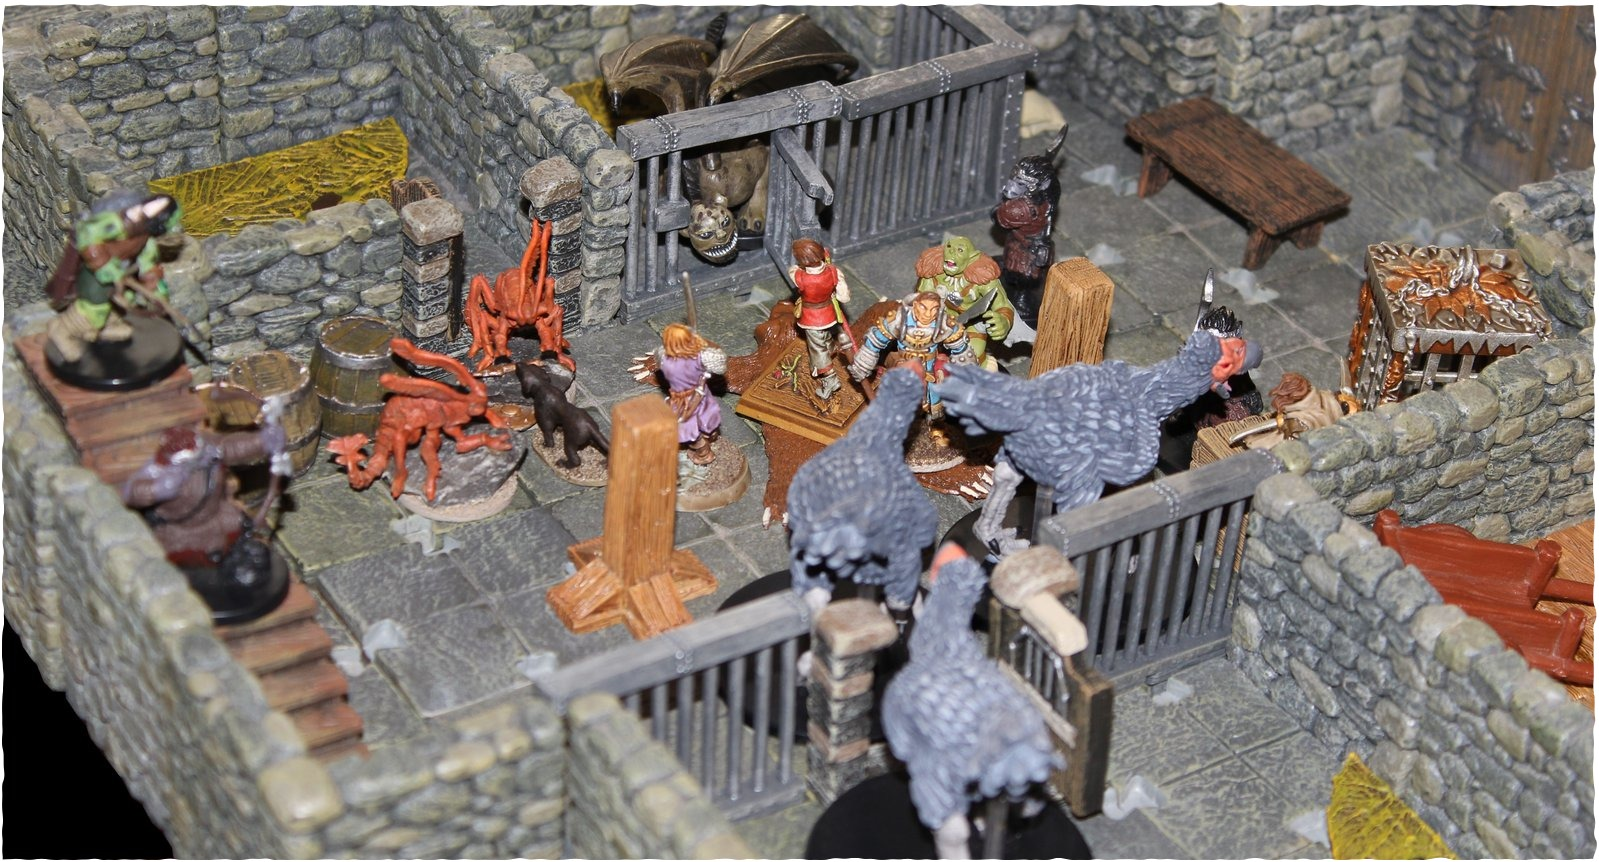
\includegraphics[width=0.4\textwidth]{images/Orc-ambush-in-Urgir-593345070_mod.jpg}
	\caption{Orc ambush in Urgir}
	\label{fig:Orc-ambush-in-Urgir-593345070}
\end{figure}

After a few rounds of healing the party explores upstairs. There is no sign of the building's proprietor Hobar, his bedroom has been ransacked and a small book lies open on his desk, with several sheets of scribbled notes on the side. The book itself is written in code and the notes are someone's failed attempt to make sense of the secret writing. Quint relishes at the challenge to decipher it and starts studying the strange letters. It takes him little over an hour to break the code and read the notes, obviously the work of the Shoanti spy.\\

The log contains all kinds of data on the orcs in Urgir. It confirms that Grask Uldeth, the orc overlord, is seated firmly on the throne, in a way that few of his predecessors ever did. He's been in power for over two decades and has used these years to plant his own pawns in the other orc clans to strengthen his influence. His many, many children have been married off to countless sons and daughters of other orc warlords. He controls an army of over 7,000 strong in Urgir and can call to arms at least double and likely even thrice this number from the other tribes in a relatively short amount of time.\\

The book also focuses on Uldeth's decision to allow {\itshape pinkskins} in the city. This policy started about nine years ago and has proven very successful: the coffers have never been so full and there is a steady supply of weapons, magic and knowledge. The orc leader has also appointed a human pathfinder as his councilor recently, probably to aid him in his efforts to unearth hidden dwarven treasures and secrets which might still be buried under the former sky citadel. The pathfinder's talent for exploration and keen archeological insight will certainly be useful in this endeavor. The most recent notes in the book mention someone named Wyrnan Korch, the Purple Worm, a person of some interest in the church of Rovagug, the Rough Beast, god of the orcs. Korch has been spending more time in the seedier parts of town lately, gathering mercenaries and allies. According to the log he is searching for the Key of Koldukar (the ancient dwarven name of Urgir). This key is rumored to provide access to unknown and unopened dwarven tunnels under the city. In the hands of a spy such a key would be of immense worth, allowing him to move about unseen from one side of the city to the other. The writer of the log decides to shadow Wyrnan Koch. His final notes includes a sketch of the temple of Rovagug; an arrow points to the southern corner of the building. It reads: {\itshape``Purple Worm entered here through secret door}''.\\

When the companions head back down to question the prisoner, they notice that little Uri has disappeared without a trace. The front door stands slightly ajar. Quint addresses the caged orc, pretending to be an agent of Arnois Belzig, Uldeth's new pathfinder advisor. The orc admits that he and his men were stationed here after they helped 'arrest' the spy who lived here. They were to ambush any of the spy's contacts, so when a group of pinkskins walked in, he naturally assumed that they conspired with the spy. When Quint asks the prisoner where the temple of Rovagug is situated, he wonders why Belzig's agents would not know something so trivial. Balian thinks the orc has served his purpose and silences him.\\

The companions return to the streets, feeling ill at ease at the thought that Uri might have betrayed them. The orc child knows where they are staying and witnessed how the killed several orcs in Hobar's house. If he has decided to snitch to the guard, the party is not safe here anymore. As they retrace their steps through the city to the market square, they scout for a good place to lay low for the night, but no obvious hide-out turns up. At one point, while still walking through the all-orc district, a passer-by notices Balian, shouts at him and moves in to pull back his hood. The ranger reacts immediately by punching the assailant in the face. Only then does he see that the orc was actually a woman. The ranger pulls his hood even closer over his head and picks up the pace before other bystanders join in. When they finally get back to the market, Puk sneaks ahead to assess the situation. The rogue notices several Urgir guards at the {\itshape Pinkhouse} , asking questions. Other guards are making inquiries on the market square. The heroes try to blend in for a while, but when the guards come too close, they decide to move. Quint addresses a random orc servant at one of the stalls and asks him for the way to the temple of Rovagug. After receiving directions the bard casts  {\itshape memory lapse} on the orc, so he won't remember the conversation. Much of this adventure was inspired by 